\documentclass{article}
\usepackage[english]{babel}
\usepackage[utf8]{inputenc}
\usepackage{fullpage,latexsym,picinpar,amsmath,amsfonts,graphicx,array,longtable,verbatim,fancybox,tikz,epstopdf,forloop,titlesec,fancyhdr,fancyvrb,amssymb,mathtools}
\usepackage[edges]{forest}
\usetikzlibrary{shapes.geometric, arrows,graphs,arrows.meta,graphs.standard,automata,positioning,calc,arrows.meta,decorations.markings,quotes}
\tikzstyle{arrow} = [thick,->,>=stealth]
\tikzstyle{arrowl} = [thick,->,>=stealth, bend left=15]
\tikzstyle{arrowr} = [thick,->,>=stealth, bend right=15]
\tikzstyle{arrowll} = [thick,->,>=stealth, bend left=35]
\tikzstyle{arrowrr} = [thick,->,>=stealth, bend right=35]
\tikzstyle{arrowlll} = [thick,->,>=stealth, bend left=55]
\tikzstyle{arrowrrr} = [thick,->,>=stealth, bend right=55]

\usepackage[headheight=20pt, headsep=0.15in, margin=0.7in, top=1in, bottom=1in, left=1in, right=1in,]{geometry}

\pagestyle{fancy}
\fancyhf{}
\rhead{\fancyplain{}{FIRST LAST}}
\lhead{\fancyplain{}{COURSE -- HW -- DATE}}

\rfoot{Page \thepage}
\renewcommand{\headrulewidth}{1pt}

\begin{document}

\noindent \textbf{0. DISCLAIMER}

I am by no means an expert so they are bound to be mistakes or anti-patterns or bad practices. This is just suppsoed to be a template to take and use with some demos and examples of stuff I found useful for homework and other things. Hope yall find this useful!

For starters, why not make a question macro that auto increments the question number? good question, i just didnt feel like doing that :shrug: sorry

\noindent\rule{\textwidth}{0.5pt}

\noindent \textbf{1. Here is a question }

Not really, but here are some math things!

Using \verb+$+ means you can write math stuff inline, where as using \verb+$$+ places it on a new line with some vertical spacing and horizontal alignment.

Here is an inline demo: $f(x)=x^{2}$

Here is a newline demo:

$$ f(x) = x^{2} $$

We can use \verb+\begin{align}+ to number the lines (and align at the \verb+&+) and center!
\begin{align}
    \sum_{i=0}^{n} \frac{1}{i} &= 0 + 1 + 2 + \hdots + n-1 + n \\
    &= \frac{n(n+1)}{2} \\
    \text{text before align $|$}&\text{$|$ text after align}
\end{align}

We can also use \verb+\underset+ and \verb+\overset+ on the summation

\begin{align}
    \underset{i=0}{\overset{\infty}{\sum}} 
\end{align}

What is the difference? it is that we can use the under and oversets on $\overset{a}{\underset{b}{\text{text}}}$ 
vs
$\text{text}_b^{a}$ 

using \verb+$\overset{a}{\underset{b}{\text{text}}}$+ vs \verb+$\text{text}_b^{a}$ +

Note the use of the dollar signs meaning we are doing some inline math text

We can remove the numbers by doing \verb+\begin{align*}+ or by doing \verb+\nonumber+ on a single line.

\noindent\rule{\textwidth}{0.5pt}

\noindent \textbf{2. QUESTION ABOUT GRAPHS }

Me and Zubair Qazi made a video about graphs

see here https://www.youtube.com/watch?v=8AOTWEcaAjg

But here is a demo

\centerline{\large Graphs in \LaTeX}

% We want to construct a directed graph from the following table
%    A   B   C   D   E
% A  0   5   6   3  -4 
% B  x   0   x   1   7
% C  x   4   0   x   x
% D  x   x   -5  0   x
% E  x   x   3   6   0

% We want to center the graph in the middle horizontal space. 
% Center here refers to horizontal center, not center of page
% Think of this as the center option when formatting text in Google Docs or Microsoft word

\begin{center}
    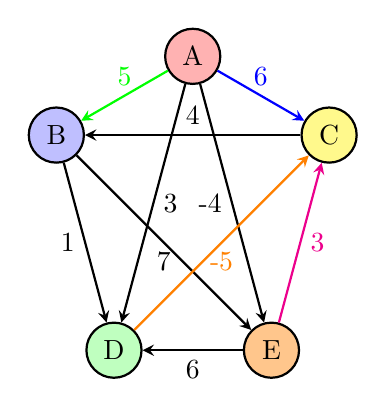
\begin{tikzpicture}[roundnode/.style={circle,draw,fill=green!25,thick,minimum size=7mm},]
        % \node [options] (var) at (x,y) or (theta:r) {label};
        %\node[roundnode,fill=COLOR!tone]
        \node[roundnode,fill=red!30] (0) at (90:2) {A};
        \node[roundnode, fill=blue!25] (1) at (150:2) {B};
        \node[roundnode,fill=yellow!45] (2) at (30:2) {C};
        \node[roundnode] (3) at (240:2) {D};
        \node[roundnode,fill=orange!45] (4) at (300:2) {E};
        
        % A -> B(5), C(6), D(3), E(-4)
        % \draw (from) to (to);
        % \draw[..., color]
        \draw[arrow,green] (0) edge node[above] {5} (1); % A -> B(5)
        \draw[arrow,blue] (0) edge node[above] {6} (2); % A -> C(6)
        \draw[arrow] (0) edge node[right] {3} (3); % A -> D(3)
        \draw[arrow] (0) edge node[left] {-4} (4); % A -> E(-4)    
        
        % B -> D(1), E(7)
        \draw[arrow] (1) edge node[left] {1} (3); % B -> D(1)
        \draw[arrow] (1) edge node[below] {7} (4); % B -> E(7)
    
        % C -> B(4)
        \draw[arrow] (2) edge node[above] {4} (1); % C -> B(4)
    
        % D -> C(-5)
        \draw[arrow,orange] (3) edge node[below] {-5} (2); % D -> C(-5)
    
        % E -> C(3), D(6)
        \draw[arrow,magenta] (4) edge node[right] {3} (2); % E -> C(3)
        \draw[arrow] (4) edge node[below] {6} (3); % E -> D(6)
    \end{tikzpicture}
\end{center}


\noindent\rule{\textwidth}{0.5pt}

\end{document}